% Figures: scripts/render_delta_maps_of12.py --all, from results/wing_maps_of12/, promoted
% into fig/. Six of the nine rendered maps are used here: Cp and the SIGNED Cf for each
% condition. The |Cf| magnitude maps are rendered but NOT carried, because a magnitude cannot
% express reversed flow and the signed field is strictly more informative on the one question
% these figures exist to answer.
\section{Surface differences on the wing}
\label{sec:deltamaps}

\textbf{Purpose.} Section~\ref{sec:app:sections} cuts the wing at five stations. This section
gives the same comparison over the whole surface at once: the baseline field, and each
candidate minus the baseline, on the upper and lower surfaces together. Twelve panels per
quantity per condition, so a feature can be located in span and chord at the same time rather
than inferred from five slices.

\textbf{A difference between two separately meshed wings needs a common support.} The wings
are meshed independently and share no cells at all: SWB carries $11{,}334{,}640$ surface
triangles against SWC's $11{,}356{,}180$, and no face of one corresponds to any face of the
other. A cell-to-cell subtraction therefore does not exist. Every face is instead binned onto a
common $(\eta, x/c)$ grid of $240 \times 320$ cells, area-weighted, with upper and lower
surfaces binned separately using the flag each export carries. That grid is the only support on
which a difference between these two wings is defined, and $76{,}797$ of its cells are filled
on both surfaces.

\textbf{The panels are drawn on the planform, not on the grid.} An $(\eta, x/c)$ image is a
rectangle, and a rectangle silently asserts a rectangular wing to any reader who does not stop
to read the axes. Each bin therefore carries its physical position and the panels are drawn on
the true swept and tapered planform, matching Figure~\ref{fig:geom:displacement} so the two can be read
against one another. Span runs left to right with the root at the left, $x$ increases upward, so
the leading edge is at the bottom. The drawn planform reproduces the registered wing to
$0.18$~per~cent in root chord ($0.6403$~m against $0.639125$), $0.2437$ against $0.238$ in
taper, and $1.0036$~m of leading-edge sweep. It is a canvas for a field, not a measurement of
the planform.

\textbf{What the figures carry.} Column~B is the baseline's own absolute field on its own scale.
The five candidate columns are candidate minus baseline on ONE shared scale, set at the
$99.5$th percentile of $|\Delta|$, so their magnitudes are comparable by eye across columns.
Blank cells are cells no face landed in, and are never zero. Every panel title carries that
case's $C_D$ in counts, its $\Delta C_D$ against the baseline of the same condition, and its
$L/D$, read from the same \texttt{rans\_forces\_current.json} harvest as the tables in
Sections~\ref{sec:cr} and~\ref{sec:cruise}, so a figure and a table cannot disagree. Each wing is
at its own trimmed incidence at the common target $C_L$, so every comparison here is at MATCHED
LIFT.
\textbf{A difference forward of the hinge is lineage, not morphing.} The candidates are not
identical to the baseline ahead of the commanded region. Measured on the placed surfaces in
absolute coordinates, C, F, H and M all depart from the baseline by the same amount, $0.316$,
$0.184$ and $0.079$~mm at $\eta = 0.60$, $0.80$ and $0.95$, and by exactly zero at
$\eta = 0.40$ and inboard; W departs further and differently, $0.366$, $1.171$ and $0.292$~mm.
Four candidates sharing one forward shape that the baseline does not is the baseline-lineage
difference of Section~\ref{sec:geom:lineage} appearing in the meshed surfaces, and it does not
cancel in a
baseline-to-candidate difference because the two sides sit on different lineages. It is small,
$2.6$~per~cent of the aft displacement at $\eta = 0.80$, but any faint forward feature in the
candidate columns should be read as lineage rather than as an effect of the morph.

\textbf{Null.} Differencing the baseline against itself returns exactly zero in every filled
cell, for every binned quantity and all three conditions, $76{,}797$ cells each. The renderer also
refuses to difference across operating points: it compares condition, Mach, $U_\infty$, grid
size and registered semispan between every pair before subtracting, and stops rather than
differencing unlike states.

\subsection{Pressure}
\label{sec:deltamaps:cp}

At Condition~CR the candidates are almost free. The pressure differences are confined to the
commanded region and are small. The trimmed drag behind each panel is Table~\ref{tab:perf:cr},
and the differences there are small beside the cruise ones but they are not scatter: the
systematics this report quantifies, in Section~\ref{sec:qv:counts}, total at most
$0.024$~counts, being window drift of $0.0014$ to $0.0028$~ct and a trim-residual effect of at
most $0.021$~ct. Section~\ref{sec:perf:recommendation} states what a margin of this size does and
does not support.
At cruise the same geometries separate into three groups. The baseline runs $177.8$~counts at
$L/D\ 29.76$ at early cruise; W saves $0.8$, F and H cost $1.8$ and $2.2$, and C and M cost
$12.9$ and $14.6$. Late cruise gives the same order. The aft-camber candidates carry a
recompression shock on the upper surface that the baseline does not, and it shows in these maps
as a sharp spanwise band of strongly negative $\Delta C_p$ running outboard across the rear of
the wing: strongest on C and M, weaker on F and H, and absent on W.

\begin{figure}[htbp]
  \centering
  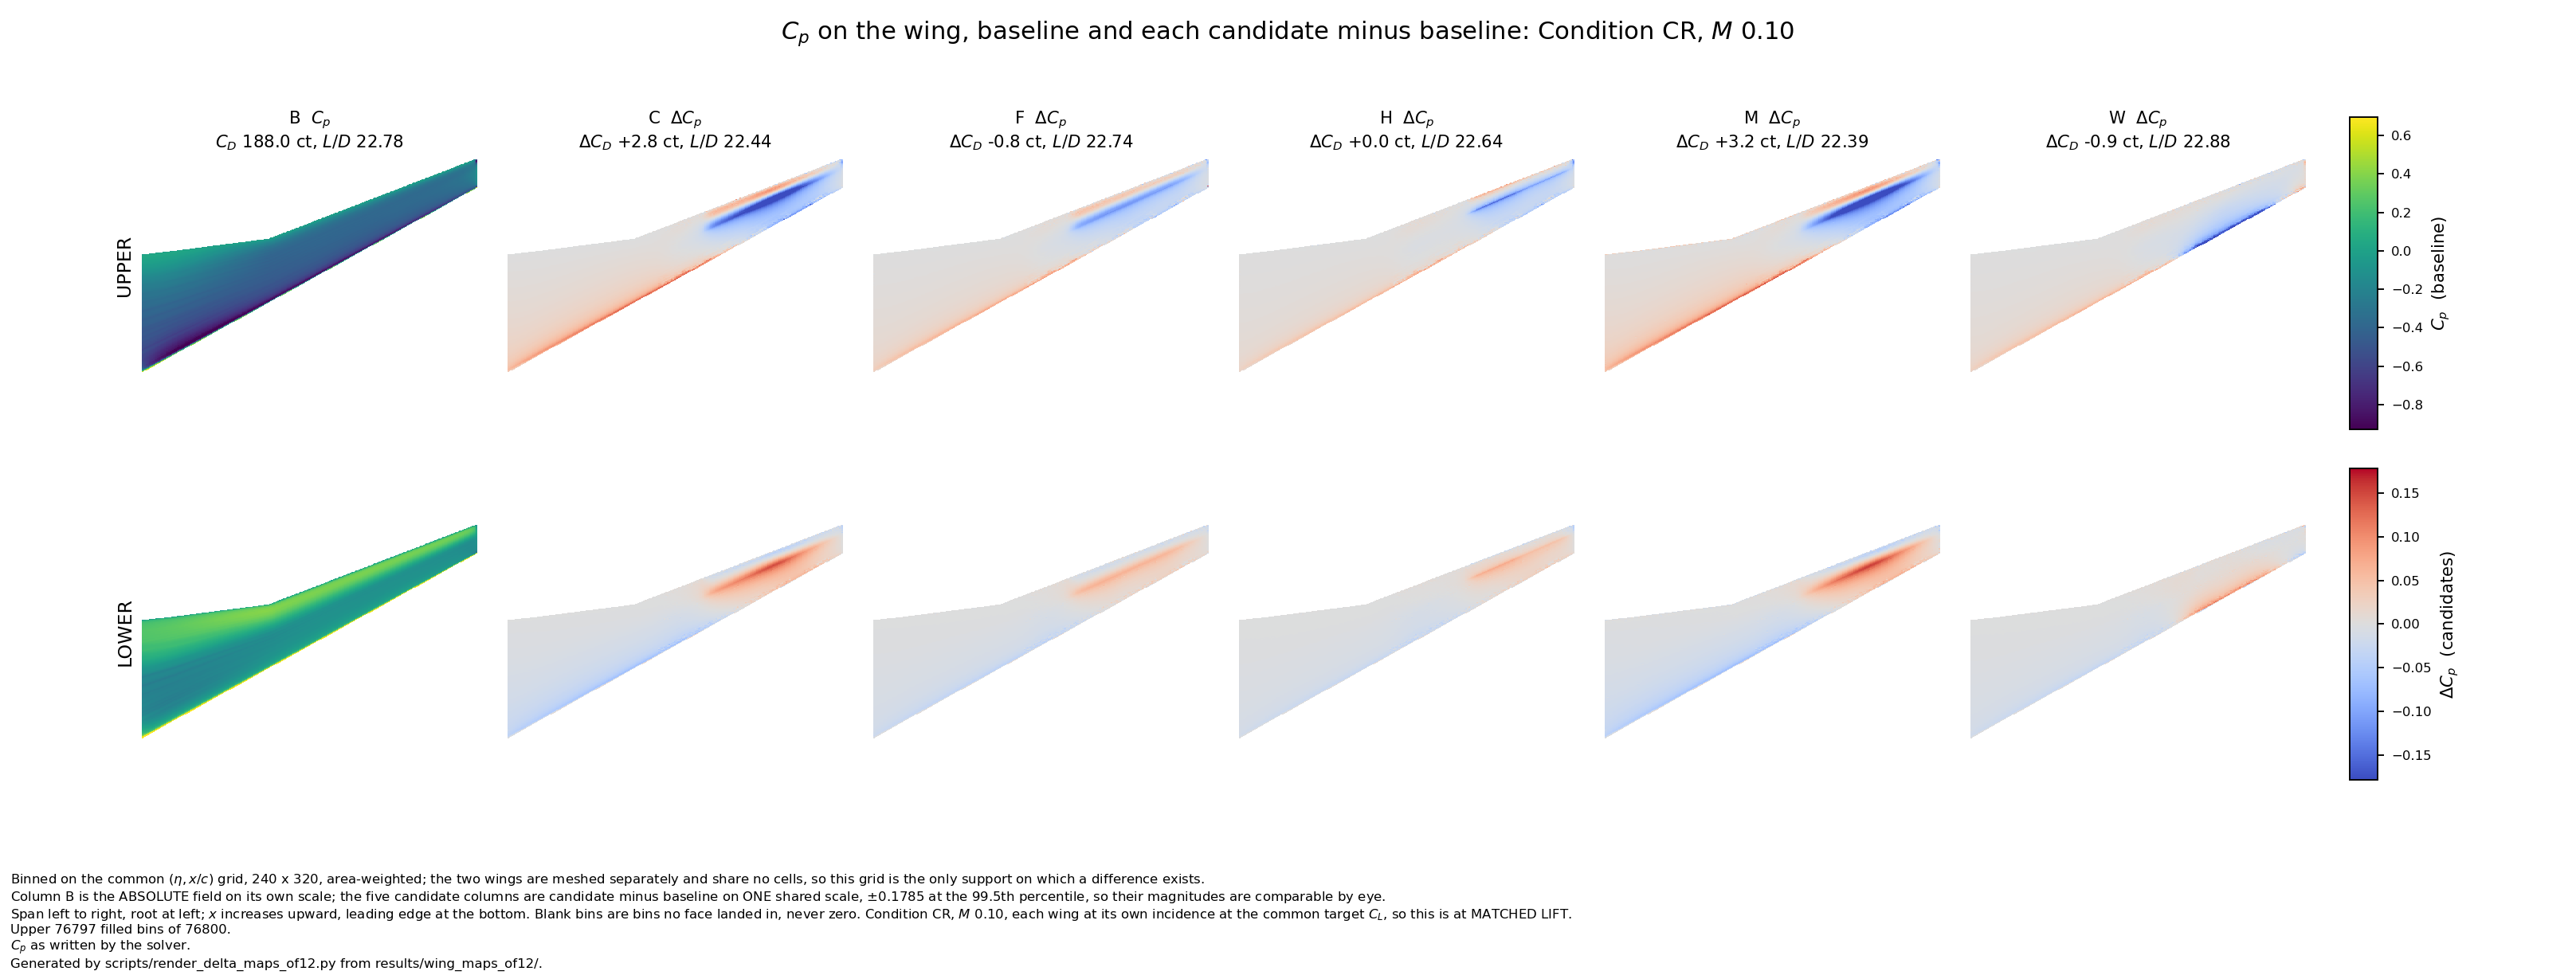
\includegraphics[width=\linewidth]{fig/delta_map_CR_cp.png}
  \caption{$C_p$ on the wing at Condition~CR, $M = 0.10$: the baseline's own field and each
  candidate minus the baseline, upper and lower surfaces. Each wing at its own trimmed
  incidence at the common target $C_L$, so this is at matched lift.}
  \label{fig:delta:cr:cp}
\end{figure}

\begin{figure}[htbp]
  \centering
  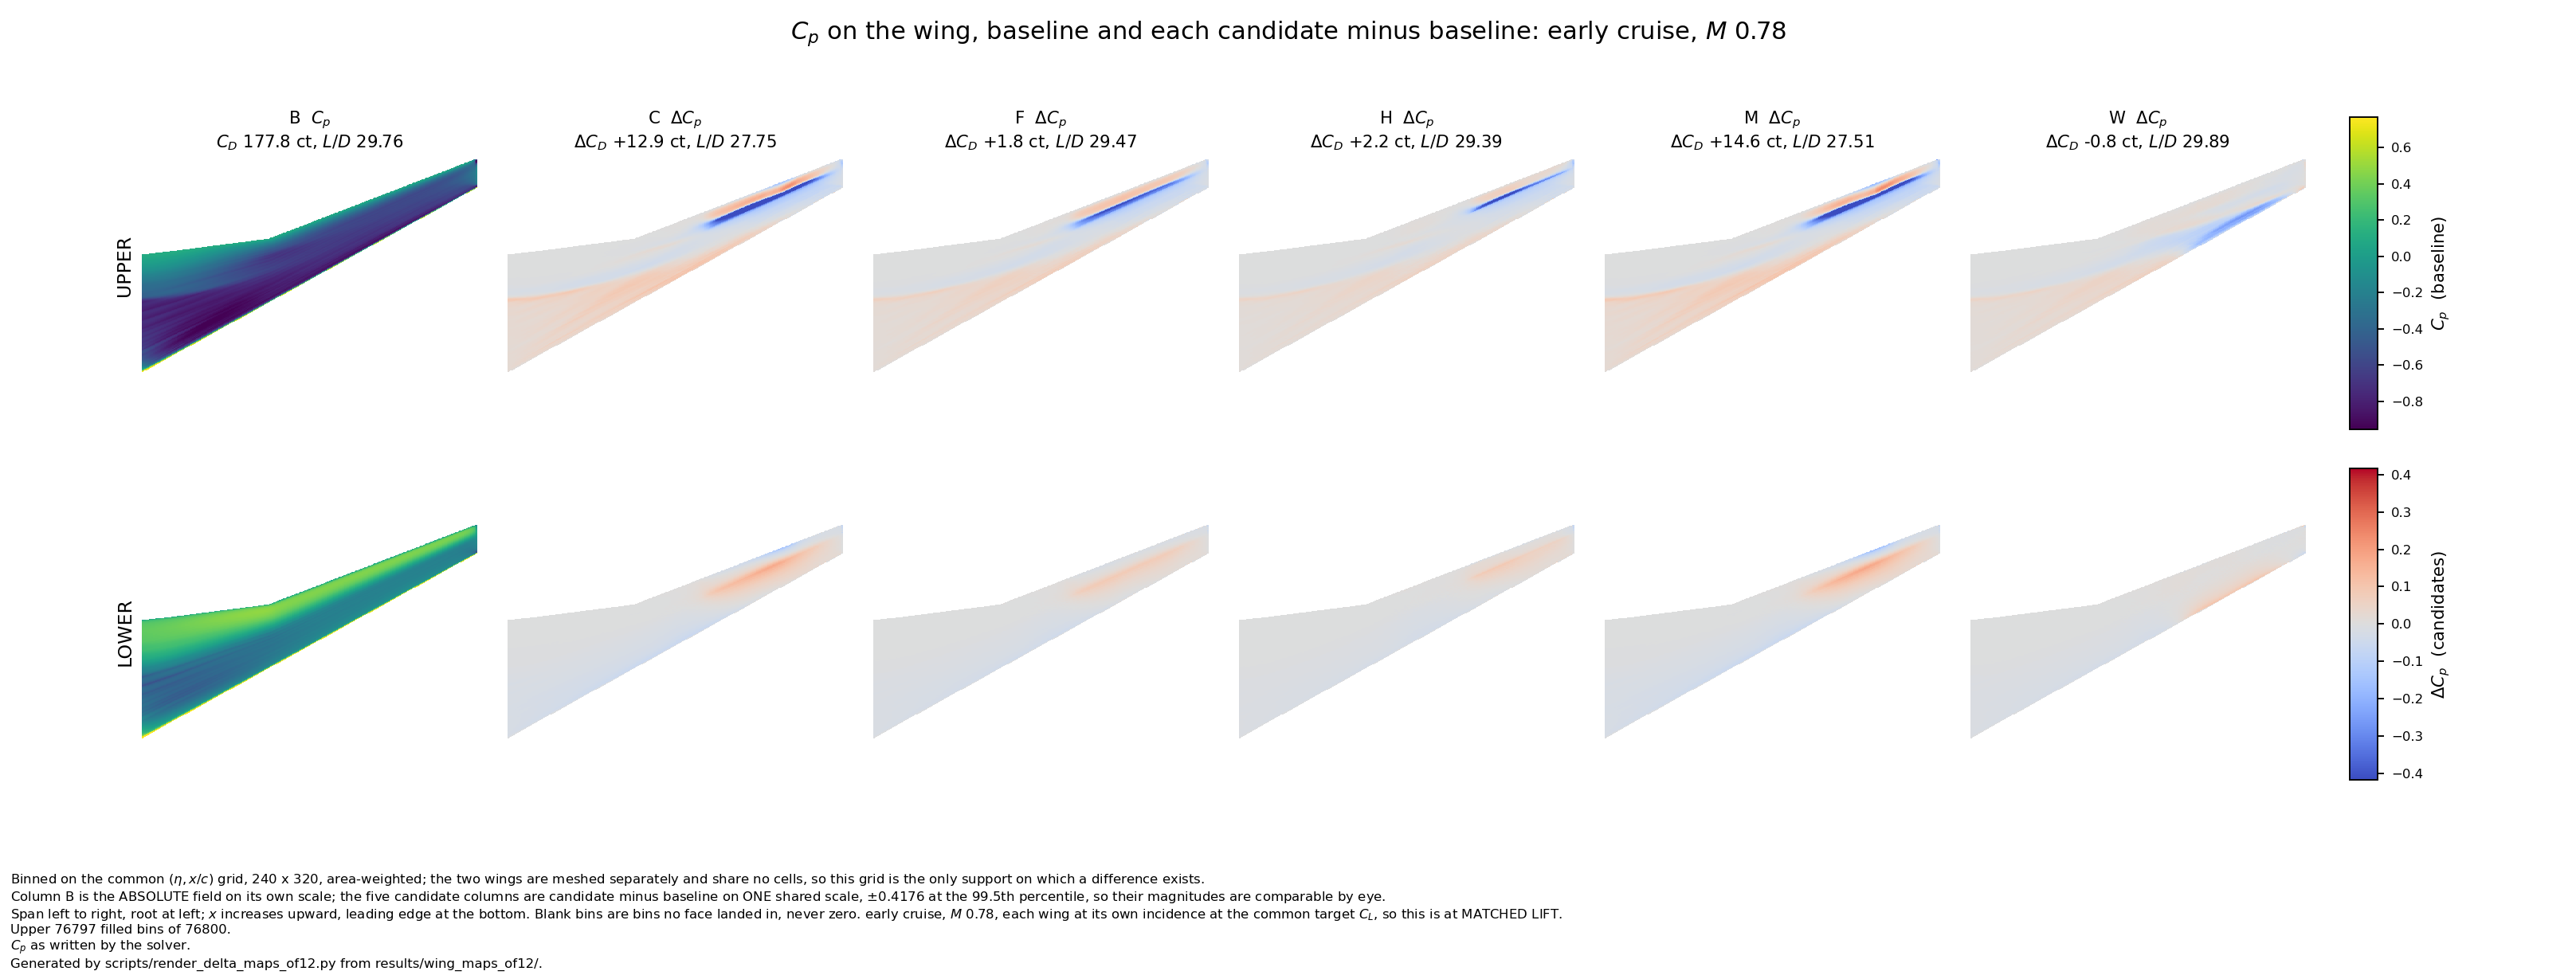
\includegraphics[width=\linewidth]{fig/delta_map_EC_cp.png}
  \caption{$C_p$ on the wing at early cruise, $M = 0.78$. The band of strongly negative
  $\Delta C_p$ across the rear of C, F, H and M is the recompression shock the baseline does not
  carry; W has none. The two most expensive candidates on drag, C at $+12.9$~ct and M at
  $+14.6$~ct, are also the two whose boundary layer does not survive that shock; see
  Section~\ref{sec:deltamaps:cfs}.}
  \label{fig:delta:ec:cp}
\end{figure}

\begin{figure}[htbp]
  \centering
  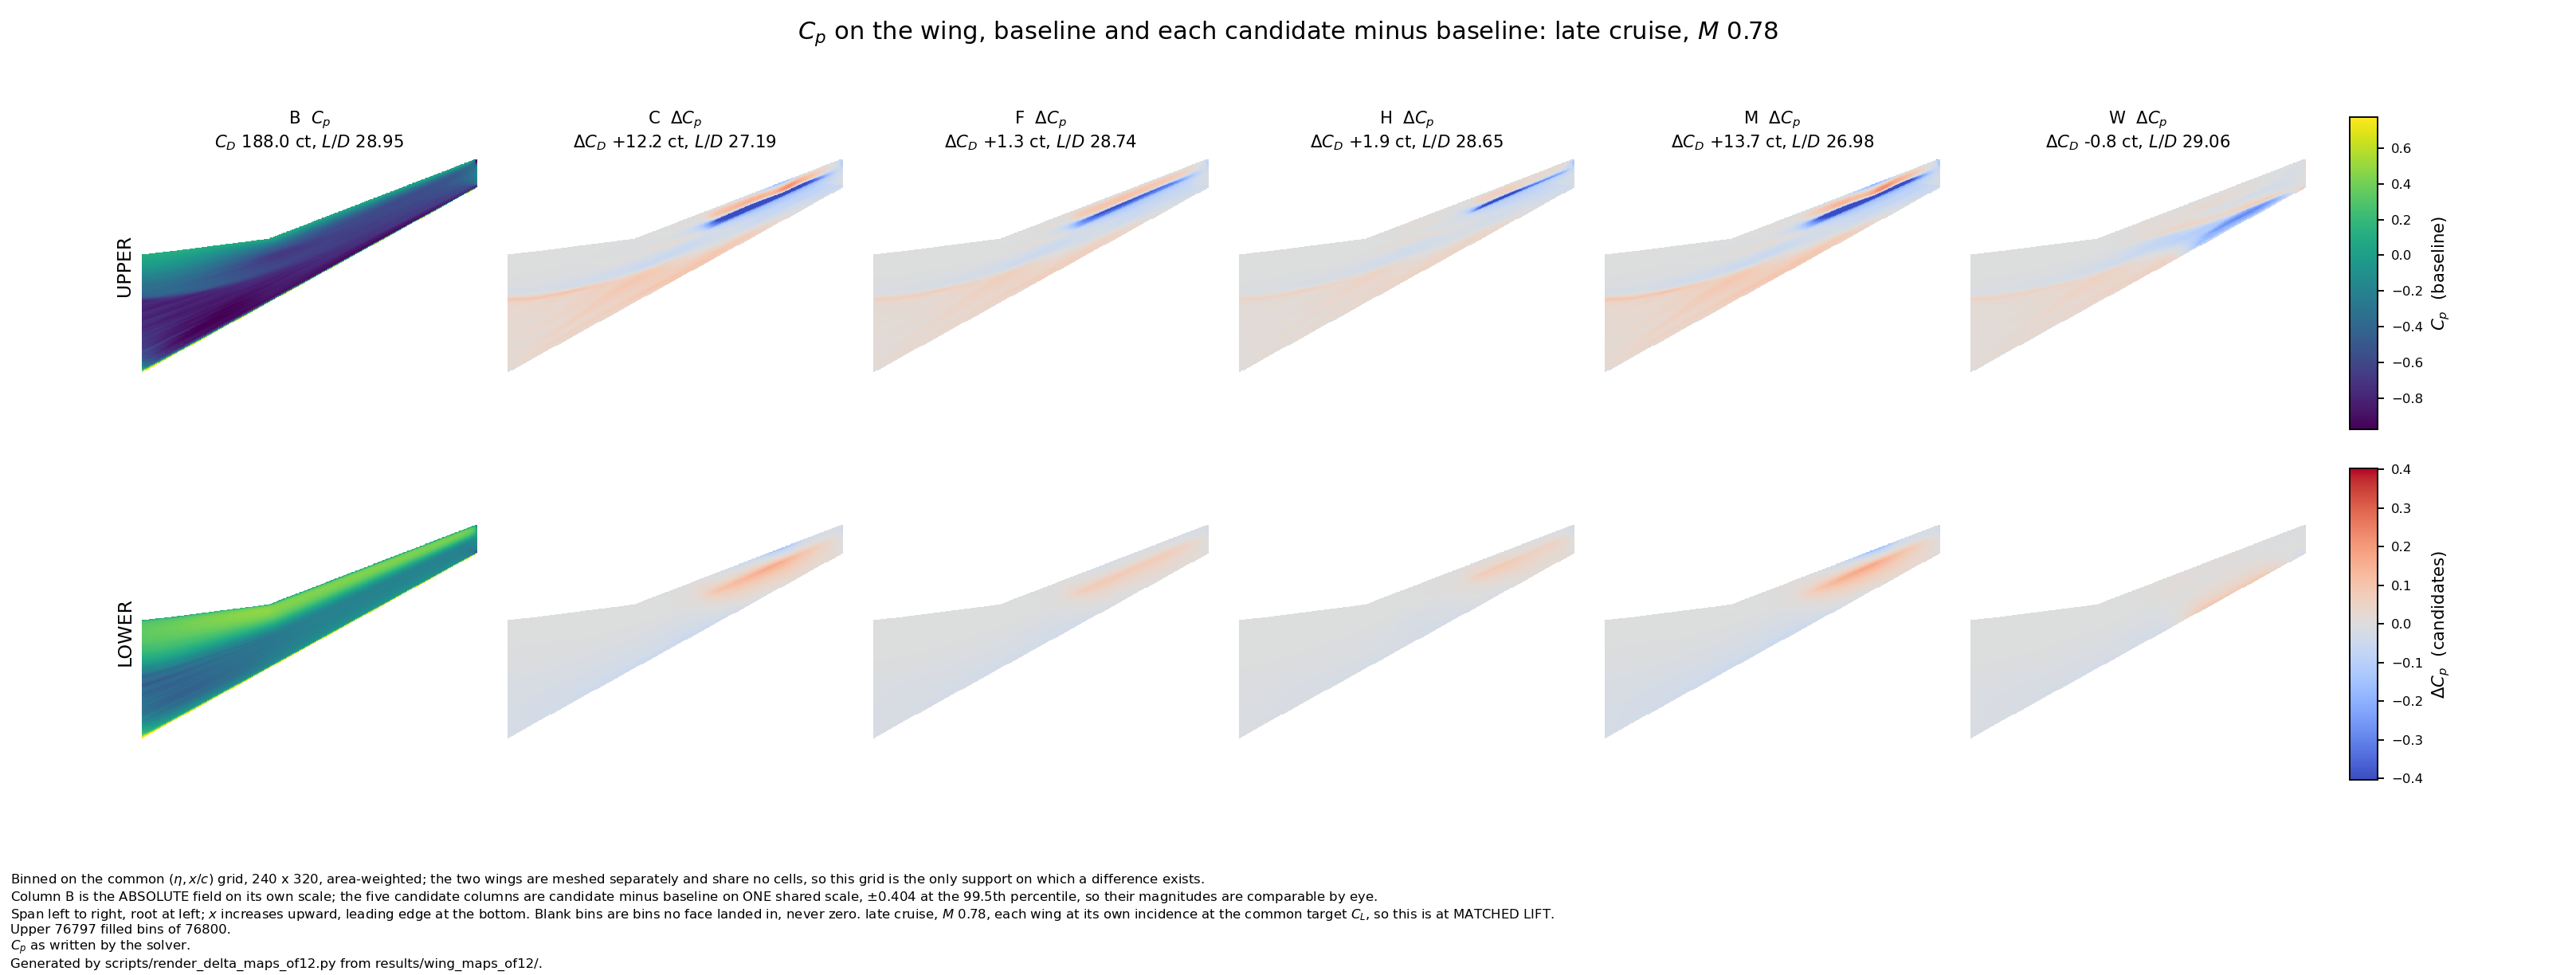
\includegraphics[width=\linewidth]{fig/delta_map_LC_cp.png}
  \caption{$C_p$ on the wing at late cruise, $M = 0.78$; as Figure~\ref{fig:delta:ec:cp}.}
  \label{fig:delta:lc:cp}
\end{figure}

\subsection{Skin friction and separation}
\label{sec:deltamaps:cfs}

\textbf{The signed component, not the magnitude.} These maps carry $C_{f,s}$, the component of
wall shear along the freestream taken from each case's own \texttt{dragDir}, so negative means
reversed flow. The magnitude $|\tau|/q$ is positive by construction and cannot express
reversal: a separated region reads as merely small and is indistinguishable from a thinned but
firmly attached boundary layer. That distinction is the whole question here, because F carries
the same shock as C and M with a visibly weakened boundary layer behind it and does not reverse.

\textbf{The sign is calibrated, never assumed.} Taken raw, the first case reported
$99.18$~per~cent of its faces reversed, which is not a separated wing but an inverted
convention: OpenFOAM's \texttt{wallShearStress} opposes the freestream where the boundary layer
is healthy. Rather than hard-code a minus sign, the sign is measured per case against faces
whose attachment is known independently of this field, namely inboard mid-chord upper faces at
$\eta = 0.15$ to $0.35$ and $x/c = 0.35$ to $0.65$. It came out one-signed on all eighteen trims,
with about $260{,}000$ calibration faces each.

\textbf{Nothing separates at Condition CR.} All six geometries reverse at most $0.013$~per~cent
of their upper-surface bins, which is $0$ to $10$ bins of $76{,}797$ at the root junction and the
blunt trailing edge, and is present on the rigid baseline too. The six are indistinguishable from
one another and from the noise floor.

\textbf{At both cruise points two candidates separate and four do not.} Measured over the whole
upper surface at early cruise: C reverses $1.520$~per~cent of its bins and M $2.122$, against
$0.004$ for the baseline, F and H and $0.000$ for W. At late cruise C reverses $1.803$ and M
$2.335$, the other four the same as at early cruise. That is a factor of some $400$ between the
two groups, on the same grid and the same code path. The lower surfaces reverse
$0.000$~per~cent on every geometry.

\textbf{The maps agree with the section cuts, on a different support.} At $\eta = 0.80$ at early
cruise the binned maps give $23.28$~per~cent of bins reversed for M and $22.97$ for C, against
the face-level section extraction's $23.86$ and $23.27$~per~cent at the same station; at late
cruise $25.16$ and $23.91$ against $25.28$ and $24.06$. Both methods return exactly zero for B,
F, H and W at both cruise points. Two independent code paths, one binning onto a common
$240 \times 320$ grid and the other counting raw faces in a band, agree to within $0.6$
percentage points and agree exactly on which cases separate. The whole-wing figures above
are smaller only because the whole wing is a much larger denominator: the reversal is real and
confined in span, not damped by the binning.

\textbf{Reduced skin friction is not separation, and the contour is what separates the two.} A
difference panel shows that the shear FELL, not that it REVERSED. The black contour is each
case's own $C_{f,s} = 0$, so flow inside it is reversed and the contour's ABSENCE is itself a
result. It is drawn only where at least $0.1$~per~cent of a surface's filled bins are negative,
because every case carries a handful of negative bins at the root junction and the trailing
edge; that threshold sits about eight times above the worst noise ($10$ bins) and fifteen times
below the smallest real signal ($1167$ bins, for C at early cruise). At Condition CR no panel
draws a contour. At both cruise points only C and M do.

\begin{figure}[htbp]
  \centering
  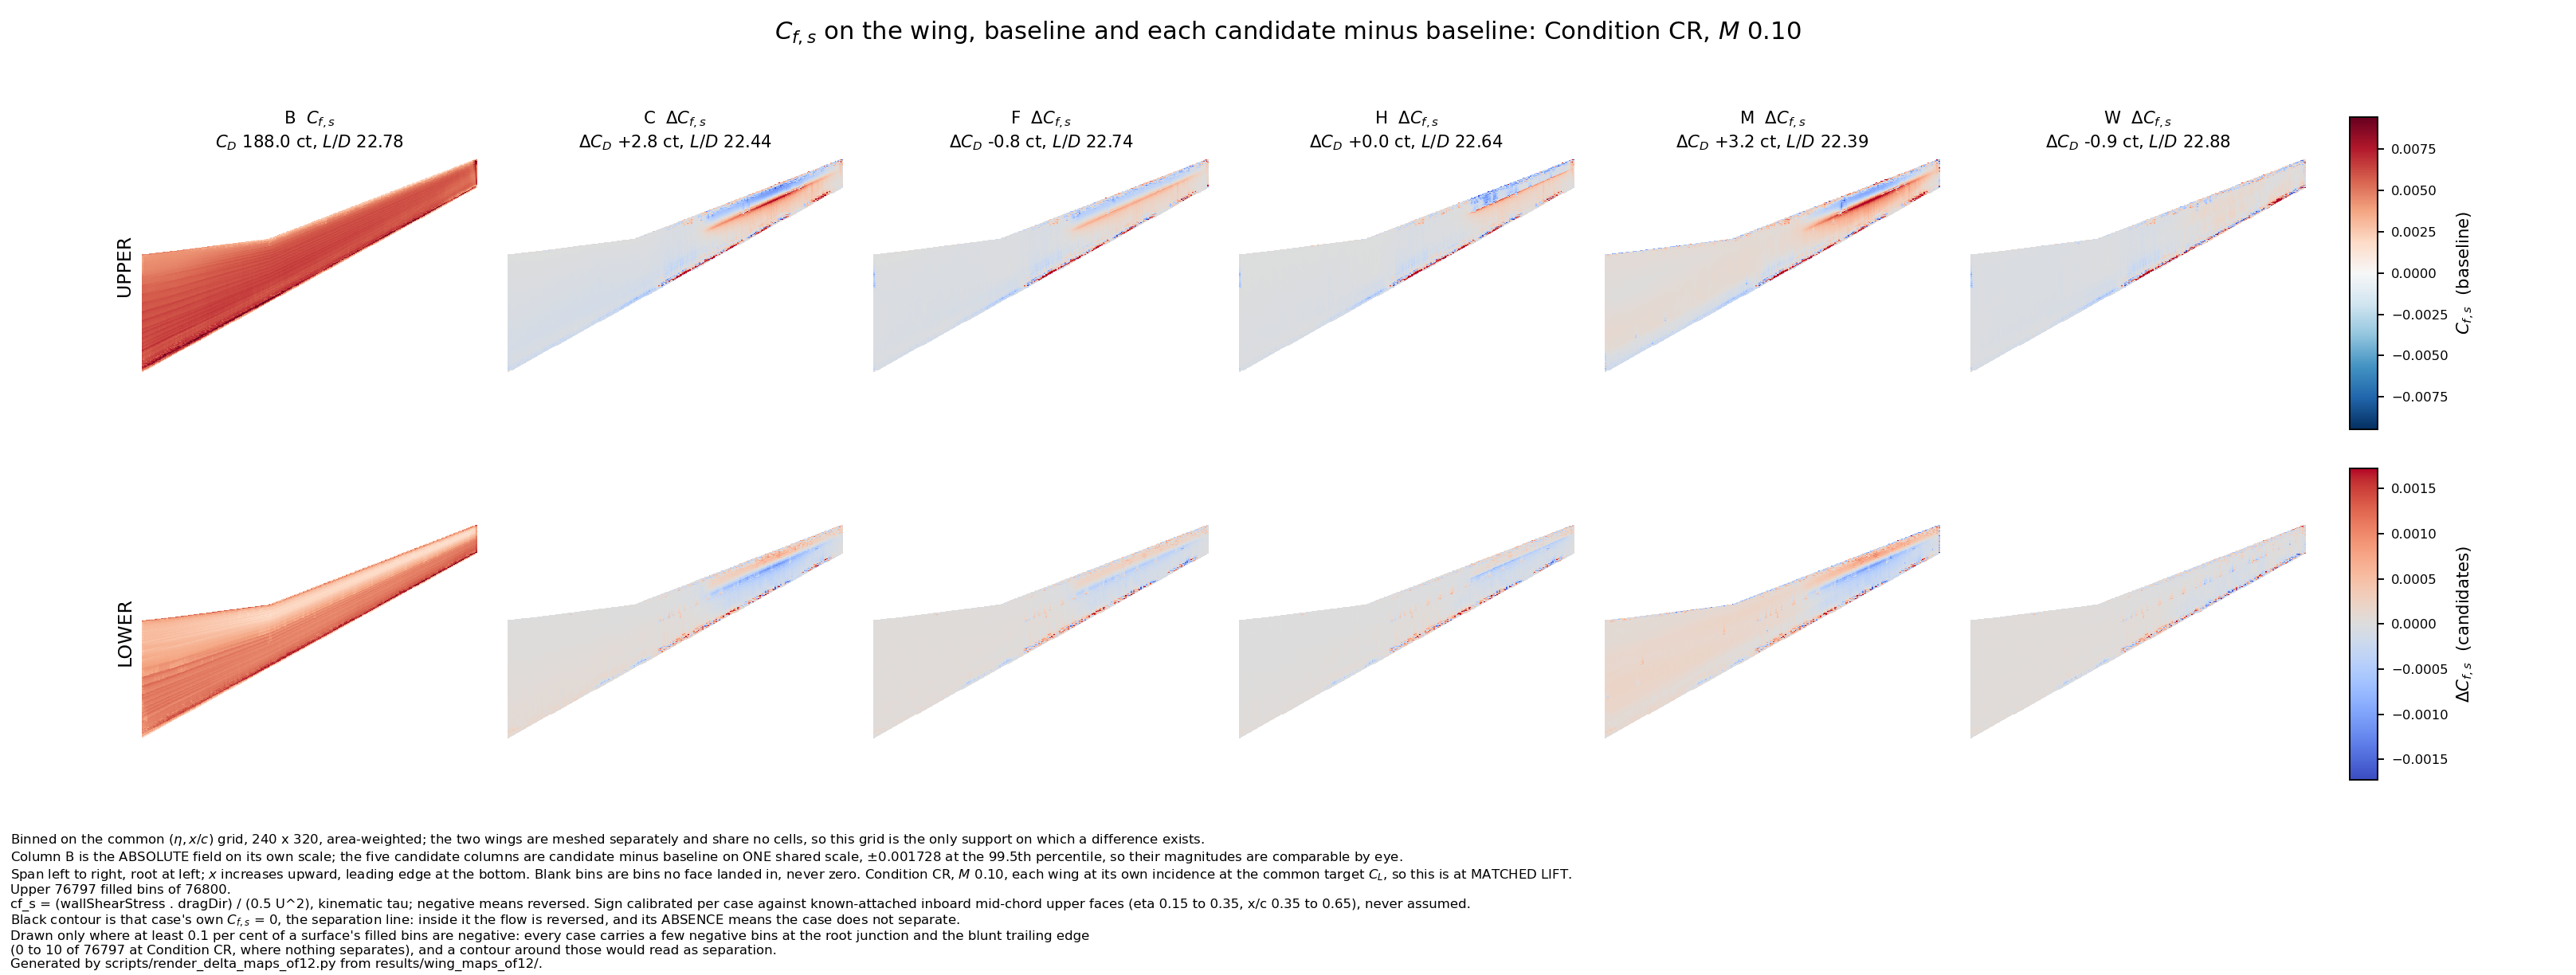
\includegraphics[width=\linewidth]{fig/delta_map_CR_cf_s.png}
  \caption{$C_{f,s}$ at Condition~CR, $M = 0.10$. No separation contour appears on any panel:
  every geometry is attached everywhere, and the candidates differ from the baseline only in the
  magnitude of the shear over the morphed region.}
  \label{fig:delta:cr:cfs}
\end{figure}

\begin{figure}[htbp]
  \centering
  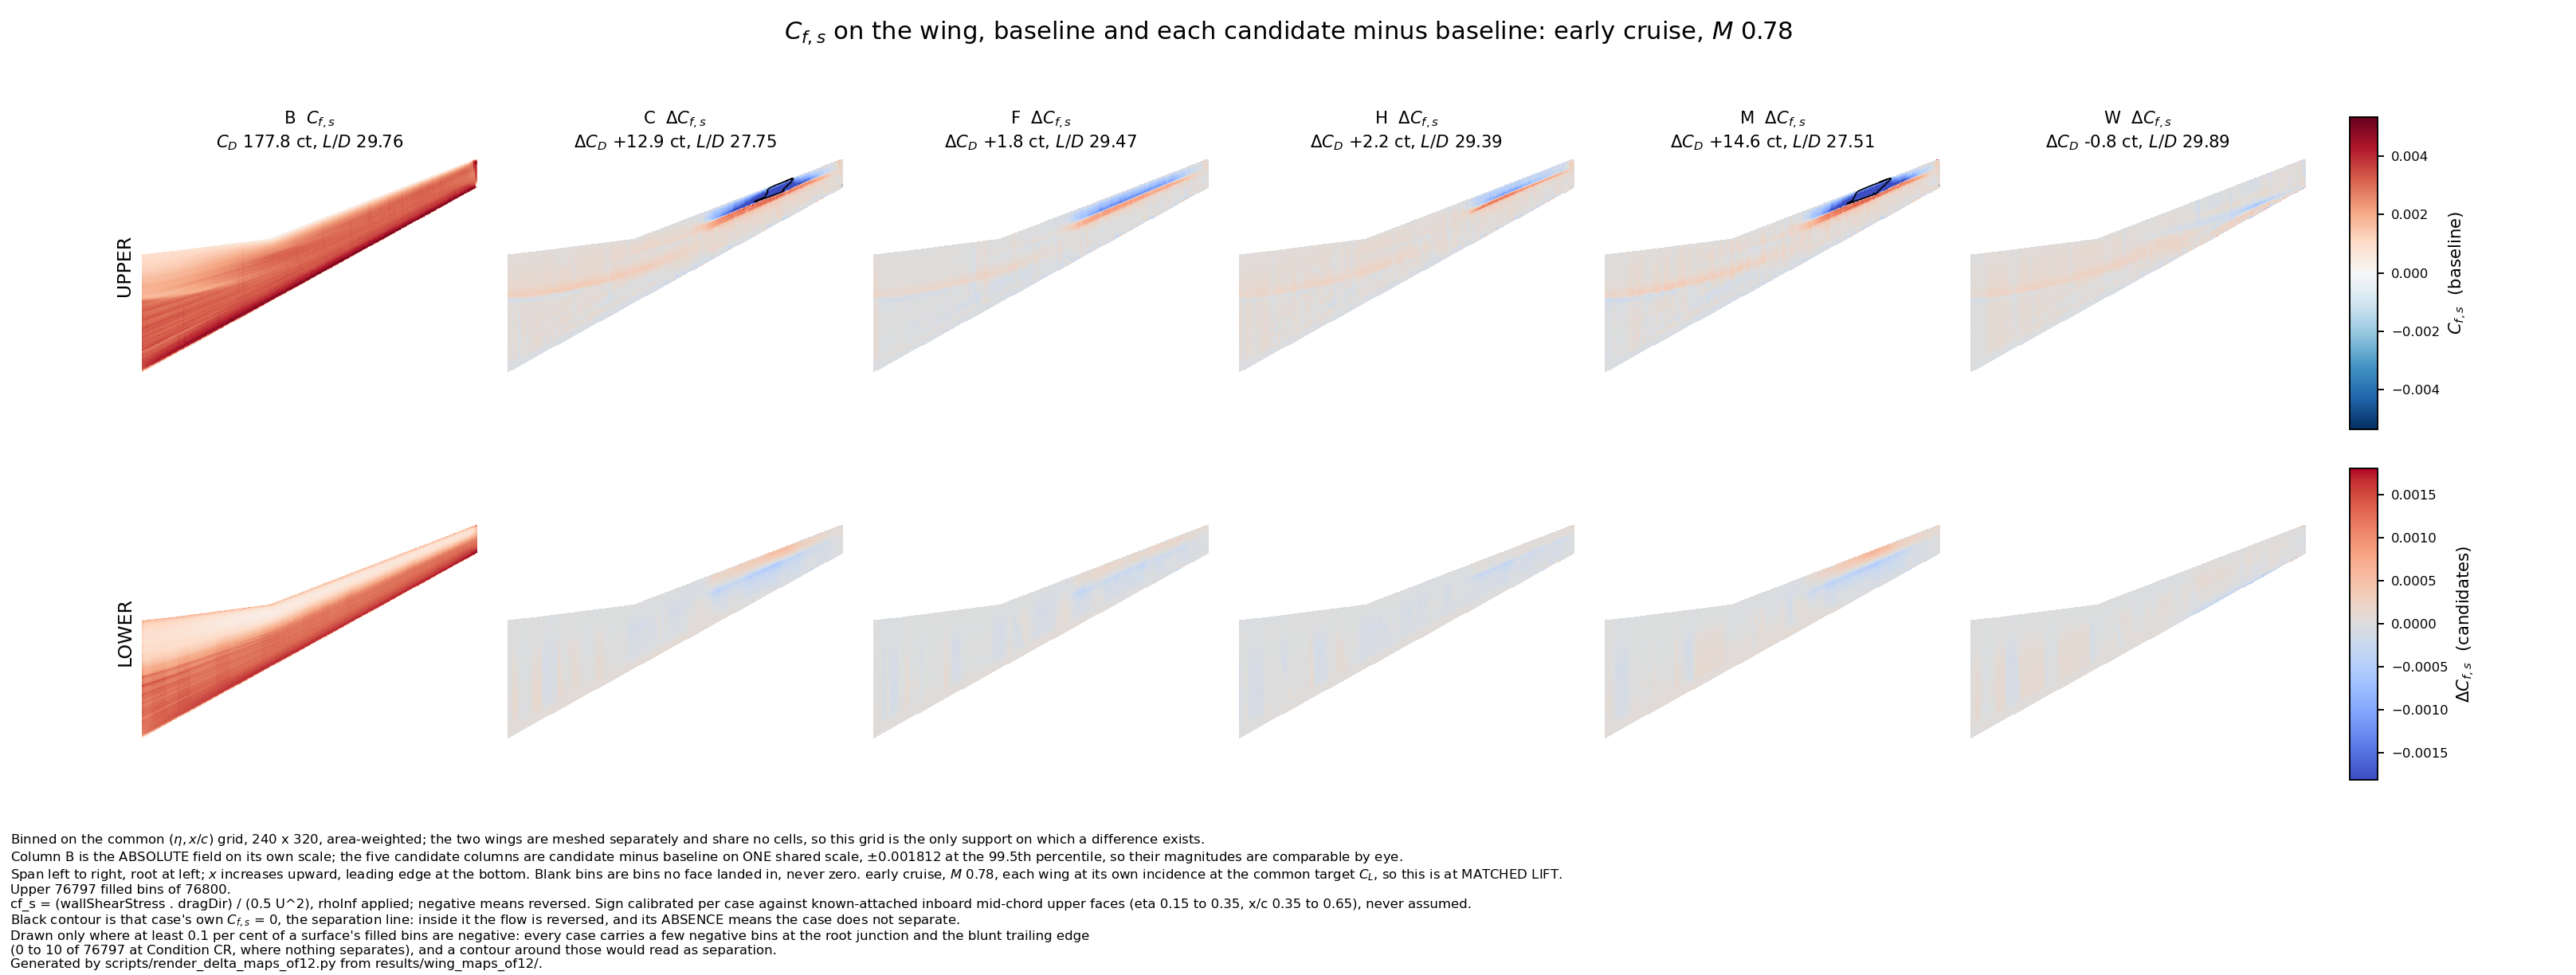
\includegraphics[width=\linewidth]{fig/delta_map_EC_cf_s.png}
  \caption{$C_{f,s}$ at early cruise, $M = 0.78$. C and M carry a closed separation contour over
  the rear outboard wing; F, H and W do not, although F and H show a fall in shear behind their
  weaker shock. The two most expensive candidates on drag, C at $+12.9$~ct and M at $+14.6$~ct,
  are the two whose boundary layer does not survive it.}
  \label{fig:delta:ec:cfs}
\end{figure}

\begin{figure}[htbp]
  \centering
  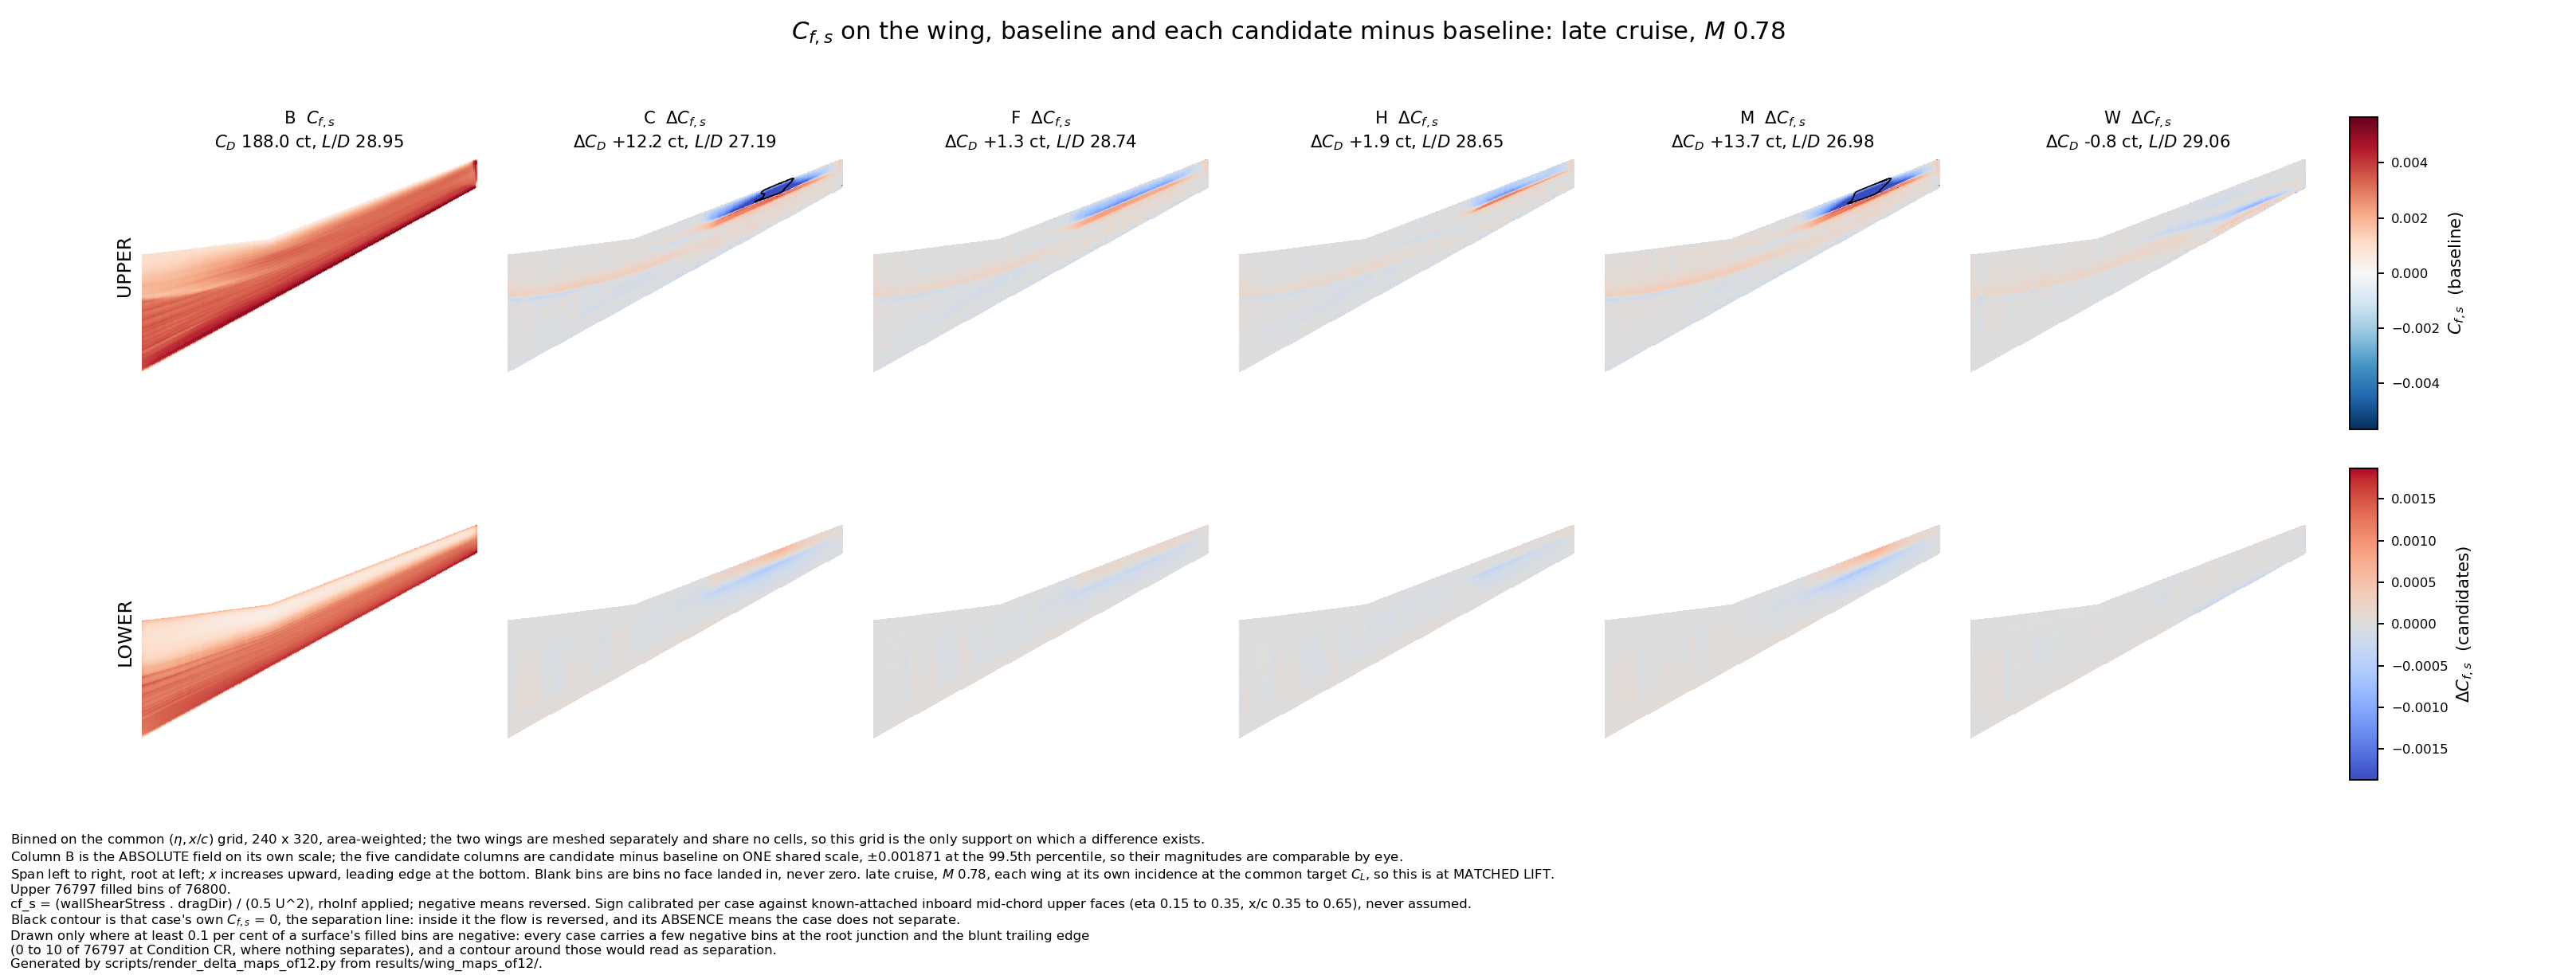
\includegraphics[width=\linewidth]{fig/delta_map_LC_cf_s.png}
  \caption{$C_{f,s}$ at late cruise, $M = 0.78$; as Figure~\ref{fig:delta:ec:cfs}.}
  \label{fig:delta:lc:cfs}
\end{figure}
